% \MakeShortVerb{\|}
% \title{Das Makropaket \texttt{folie.sty}}
% \author{Rüdiger Beck}
% \maketitle
%^^A ==========================================================================
%^^A
%^^A
%^^A ==========================================================================
% \section{Beschreibung}
% Das Paket \texttt{folie} dient dazu Overhead-Folien zu erstellen, die auf einem
% eingescannten Bild basieren.
%
% Um den Speicherplatz gering zu halten wird pdflatex verwendet, das unter anderem
% \texttt{*.png}-Dateien und \texttt{*.jpeg}-Dateien einbinden kann. Alle
% Grafiken müssen in diesem Format
% vorliegen. 
%
% Um auch Bildunterschriften und Beschreibungen durchsuchbar zu machen, werden sie
% alle im pdftex-code eingegeben, und \textit{nicht} mit der Bildbearbeitungssoftware in
% die {*.png}-Datei oder {*.jpeg}-Datei eingebunden.
%
% Zusätzliche Informationen, die die Zuhörer nicht sehen sollen, werden
% an ganz bestimmte Stellen im unteren Bereich der Folie ausgegeben. Sie können
% von hinten mit Adressaufklebern abgeklebt werden. Damit werden sie nicht 
% projeziert, sind für den Vortragenden jedoch lesbar.
%^^A
% Die Größe der Adressaufkleber ist bei mir 95\,mm x 47\,mm. Das ergibt 2 Spalten
% mit je ca. 90\,mm breite.
%^^A
% In der Kopfzeile und Fusszeile können Zusatzinformationen gespeichert werden.
%^^A
% \section{Kopf und Fußzeilen}
%^^A
% Die Kopfzeile links oben zeigt das Verarbeitungsdatum. Rechts oben erscheint
% das Lehrerkürzel (Bz) und der Dateiname der Quelldatei.
%
% Alle weiteren Felder sind editierbar.
%
% \DescribeMacro{Titelo}  
% Der Befehl |\Titelo{Text}| setzt den \texttt{Text} mitten in die
% Kopfzeile. Dieser Text dient als Überschrift.
%^^A
% \DescribeMacro{Titelu}  
% Der Befehl |\Titelu{Text}| setzt den \texttt{Text} mitten in die Fußzeile.
%
% \DescribeMacro{Fach}  
% Der Befehl |\Fach{Text}| setzt den \texttt{Text} links in die Fußzeile.
%
% \DescribeMacro{Quelle}  
% Der Befehl |\Quelle{Text}| setzt den \texttt{Text} rechts in die
% Fußzeile. Dieser Text dient zur Angabe der Quelle des eingescannten
% Bildes. Dies ist wichtig für die Suchfunktion.  
%
% \section{Einbinden von Bildern}
% \DescribeEnv{bild}
% Mit der Umgebung
% \begin{verbatim}
%    \begin{bild}{Dateiname}{Bild-Breite in mm}
%       ... Text  
%    \end{bild}
% \end{verbatim}
%
% können \texttt{*.png}-Bilder und  \texttt{*.jpeg}-Bilder zentriert eingebunden 
% werden. Der \texttt{Text} wird zentriert unter das Bild gesetzt. Er kann 
% mehrzeilig sein. 
%^^A
% \section{Zusatzinformationen}%
% Mit der Umgebung
% \begin{verbatim}
%    \begin{info}
%       ... Text  
%    \end{info}
% \end{verbatim}
%
% können Zusatzinformationen angegeben werden, die mit Adressaufklebern
% abgeklebt werden können. Der Bereich für die Zusatzinformationen ist
% 2-spaltig. Der Umbruch zwischen den beiden Spalten erfolgt automatisch so,
% dass sich der Text gleichmäßig in 2 Spalten unterteilt. 
%
% Möchte man zwischen den beiden Spalten an einer Stelle einen Umbruch
% erzwingen, kann man dies mit den Befehl \DescribeMacro{neu} |\neu| erreichen. 
%
% Um allen Text in der linken Spalte zu haben, stellt man |\neu| als letztes in
% die |info|-Umgebung.
%
%
%
%
%
%
%
%\section{Lastenheft \\ --- Ziele bei der Erstellung von \texttt{folie.sty} }
%
%Es soll eine Vorlage geschaffen werden, die Folien mit informativer
%Beschriftung (Daten, Infos, die zur Folie gehören) erzeugt


%\subsection{Dateiformate}

%\begin{itemize}
%  \item Dateiformat der Grafik: *.eps oder *.png (*.png ist vorzuziehen, da
%    meist hochaufgelöste Scans verwendet werden (geringere Dateigröße bei Scans).
%    D.h., es muss pdflatex verwendet werden (Latex kann kein *.png direkt
%    importieren). Vektorgrafik evtl. als *.eps (kann pdflatex das?)
%  \item AutoCAD (Umweg über *.eps, geht mit Gimp), Dia, Gimp, ... können *.png
%    erzeugen!
%  \item Die Beschriftung der Datei soll per Volltextsuche durchsuchbar
%    sein. Deshalb *.tex und *.pdf als Formate
%  \item Das Bild soll mittig erscheinen, mit Parameter leicht anhebbar oder
%    absenkbar.
%  \item Klappfolien: In einem Diagramm erstellte Grafik soll Deckungsgleich
%    eingeführt werden können.
%\end{itemize}


%\subsection{Erläuterungen zur Folie}

%\begin{itemize}
%  \item Die Erläuterungen sollen Text, Formeln, Bilder, etc... enthalten
%    können. Sie wird mit auf die Folie gedruckt, in 2/3 Felder, die immer an der
%    gleichen Stelle liegen. Wenn 1 Feld voll ist, springt der Text in das zweite
%    Feld.(Latex: 1 minipage erstellen, two- oder multicolumn.)
%  \item Damit die Zuhörer nicht die Erläuterungen sehen können, werden diese mit
%    undurchsichtigen weißen Klebern von Hinten überdeckt. (z. B. 2 Aufkleber
%    100x31, 3 Aufkleber(besser zu Kleben, besser zu lesen) mit
%    54x35(Zweckform)/39x50(Herma))
%  \item Textgröße so wählen, dass 2 verschiedene Klebergrößen alles abdecken.
%  \item Evtl. Markierungen zum ortgerechten Aufkleben.
%  \item Feld zur Bildunterschrift in Latex (Per Volltextsuche Durchsuchbar,
%    nicht mehr in das Bild einbinden (keine Volltextsuche)
%  \item Erläuterung evtl. in Fusszeile
%  \item Per Befehl ausblendbar: Erläuterung, ...
%  \item Um psfrag benutzen zu können, sollten auch *.eps eingebunden werden 
%    können. Dann muss jedoch gelatext werden (nich pdflatex)
%  \item bei mehrseitigen folien noch ein verlinktes Folienverzeichnis(wie geht 
%    das mit eps und png gemischt?)
%\end{itemize}

%\subsection*{Farbe}

%\begin{itemize}
%  \item Farbunterstützung (Schrift, Grafik)
%  \item Farbunterstützung ein und abschaltbar.
%\end{itemize}

%Skizze der Hochformat-Vorlage:
%\vspace{10mm}
%\begin{center}
%    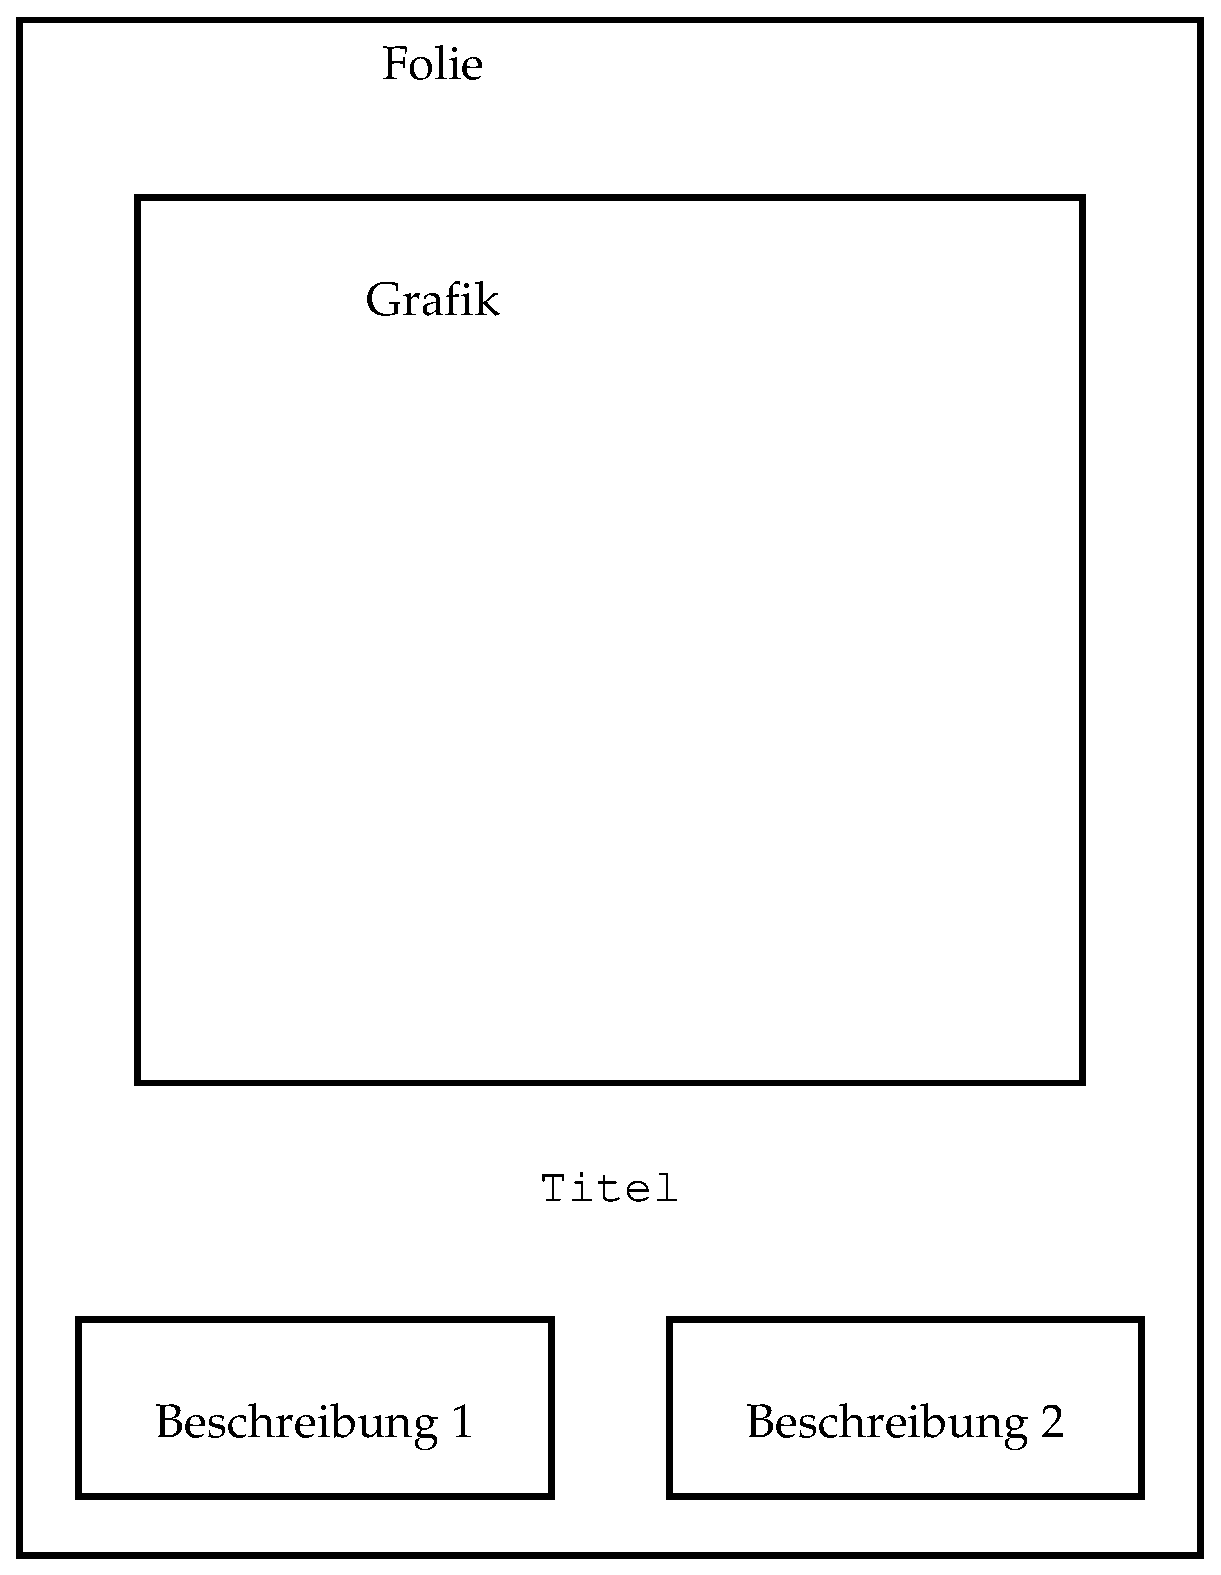
\includegraphics[width=120mm]{folie-layout}
%\end{center}
%
%
%\section{To do}
%
% Farbe ermöglichen
%
% Längen stimmen nicht überein. 100mm im tex-code ist nicht gleich 100mm gedruckt.
 
%
%^^A
% \StopEventually{}  
% ^^A ==========================================================================
% ^^A ==========================================================================
% ^^A ==========================================================================
%^^A
\newsavebox{\fach} \newsavebox{\quelle} \newsavebox{\titelo}
\newsavebox{\titelu}
% \begin{macro}{\neu}
%    \begin{macrocode}
\newcommand{\neu}{\par \newpage \par}
%    \end{macrocode}
% \end{macro}

\newcommand{\Quelle}[2][]{\sbox{\quelle}{\small #2}}
\newcommand{\Fach}[2][]{\sbox{\fach}{\small #2}}
\newcommand{\Titelo}[2][]{\sbox{\titelo}{\small #2}}
\newcommand{\Titelu}[2][]{\sbox{\titelu}{\small #2}}



% \begin{environment}{bild}
%    \begin{macrocode}
\newenvironment{bild}[3][]{% Beginn von begin
   \rule{0mm}{1mm}% Es muss was da stehen, damit \vfill tut
   \vfill
   \begin{center}
      \includegraphics[width=#3mm]{#2}
      \par \bigskip
      \bf \Large
      \begin{minipage}[t]{160mm}
      \begin{center}
}% Ende von begin
{%Beginn von Ende
      \end{center}
      \end{minipage}
      \rm
   \end{center}
   \vfill
}% Ende von Ende
%    \end{macrocode}
% \end{environment}



% \begin{environment}{info}
%    \begin{macrocode}
\newenvironment{info}{% Beginn von begin
\begin{minipage}[b][48mm][b]{180mm}
    \begin{multicols}{2}
}% Ende von begin
{%Beginn von Ende
    % es muss hier noch etwas stehen, das dann in den letzten Spalte steht,
    % wenn nur die erste Spalte genutzt werden soll
    \rule{0mm}{1mm} % ist nicht sichtbar, nimmt keinen horizontalen Platz ein
    \end{multicols}
\end{minipage}
}% Ende von Ende

%    \end{macrocode}
% \end{environment}







